\section{Theorie}
\label{sec:Theorie}
Das Geiger-Müller-Zählrohr ist eines der wichtigsten Messgeräte für ionisierende Strahlung,
insbesondere $\alpha$- und $\beta$-Strahlung, welche zu fast \SI{100}{\percent} detektiert wird.
$\gamma$-Strahlung wird nur zu etwa \SI{1}{\percent} aufgenommen,
sodass nur hohe Intensitäten mit diesem Versuchsaufbau gemessen werden sollten.

Für jedes in seinem Inneren absorbierten Teilchen erzeugt es einen elektronischen Impuls,
der anschließend durch einen Impulszähler aufgenommen wird.
Somit kann die Intensität der Strahlung bestimmt werden.

\subsection{Aufbau des Geiger-Müller-Zählrohrs}
Das Geiger-Müller-Zählrohr besteht im Wesentlichen aus einer zylindrischen Kathode in welcher ein Anodendraht positioniert ist.
Die Kathode besitzt an einer Seite ein Eintrittsfenster, durch welches die Strahlung nahezu ungehemmt eintreten kann.
Zwischen Kathode und Anode ist ein spezielles Gasgemisch unter niedrigem Druck eingefüllt.
Zwischen den Elektroden wird eine Spannung in der Größenordnung $\SI{100}{\volt}$ bis $\SI{1000}{\volt}$ angelegt.

\subsection{Funktion}
Wenn nun eines der Gasmoleküle innerhalb des Zählrohrs durch Strahlung ionisiert wird, wird das ausgelöste Elektron Richtung Anode und das ionisierte Molekül
Richtung Kathode beschleunigt. Dabei wird das Elektron so stark beschleunigt, dass es wiederum weitere Moleküle ionisieren kann.
Es kommt außerdem durch Stoßprozesse zur Erzeugung von UV-Strahlung, sodass sich die Kettenreaktion der Ladungsauslösung
auch senkrecht zum E-Feld, und somit durch das gesamte Zählrohr, ausbreiten kann.

Dies hat den Vorteil, dass dadurch so große Impulse entstehen, dass sie nicht besonders stark verstärkt werden müssen und die
Messung vergleichsweise einfach ist. Ein Nachteil ist jedoch, dass die Messung keine Information
über die Energie der Strahlung hergibt. Somit kann auch nicht mehr zwischen $\alpha$-, $\beta$- und $\gamma$-Strahlung unterschieden werden.

Ionen benötigen wesentlich länger als Elektronen, um die Kathode zu erreichen.
Das bewirkt unter Anderem, dass die Entladungslawinen nicht unbegrenz lange stattfinden, da die effektive Feldstärke
im Zählrohr abnimmt.
In diesem Zustand sind keine weiteren Ionisationen durch eingehende Strahlung mehr möglich.
Die Zeit, in der nach einem registrierten Event keine neuen Events aufgenommen werden können, wird Totzeit genannt.
Nach der Totzeit folgt ein Bereich, die Erholungszeit, in dem die erzeugten Impulse schwächer sind als zuvor.

Die Zeit, die ein Ion bis zur Zylinderwand braucht, ist in der Regel länger als die Totzeit, sodass der Effekt nicht von neuen
Strahlungsevents unterschieden werden kann und die Messung stark verfälscht.
Daher liegt ein besonderes Augenmerk auf der Vermeidung der sogenannten Nachentladungen.

Um zu verhindern, dass die Ionen, welche durch das Feld beschleunigt werden, weitere Elektronen ausschlagen,
wenn sie die Kathode erreichen, werden dem Gas vielatomige Moleküle mit vielen Schwingungsmoden zugefügt. Diese geben eines ihrer Elektronen an die Ionen ab
und werden statt ihrer zur Kathodenwand beschleunigt.
Dort können sie jedoch kein Elektron ausschlagen, sondern werden nur zu Schwingungen angeregt.

\subsection{Kenngrößen}
Wird die Anzahl der gemessenen Events $N$ gegen die am Zählrohr angelegte Spannung aufgetragen, so ergibt sich die Charakteristik
des Zählrohrs, beispielhaft in Abbildung \ref{fig:plateau}.
\begin{figure}[H]
  \centering
  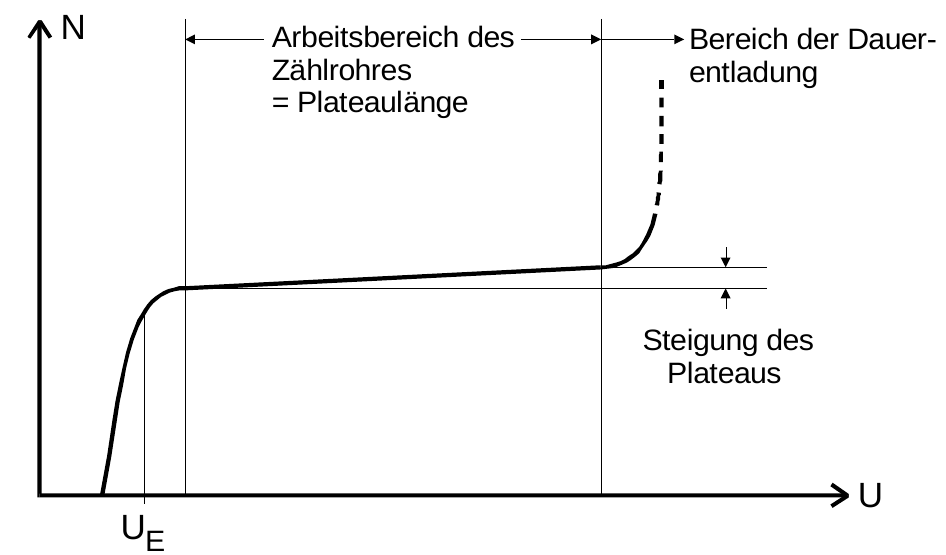
\includegraphics[width=\textwidth]{content/plateau.png}
  \caption{Charakeristik des Zählrohrs.\cite{v703}}
  \label{fig:plateau}
\end{figure}
Der lineare Teil der Chakateristik wird Plateau genannt.
Im wesentlichen wird die Steigung dieser bestimmt durch die Anzahl der Nachentladungen.
Je flacher das Plateau, das heißt je weniger die Anzahl der Events von der Spannung abhängen, desto besser ist das Zählrohr.

Die Totzeit lässt sich durch die Zwei-Quellen-Methode und über eine oszillographische Messung bestimmen.
Für die oszillographische Messung wird das Zählrohr an ein Oszilloskop angeschlossen.
Es wird für eine hohe Strahlenintensität gesorgt.
Auf dem Oszilloskop sollte ein Bild gemäß Abbildung \ref{fig:osz} erscheinen.
\begin{figure}[H]
  \centering
  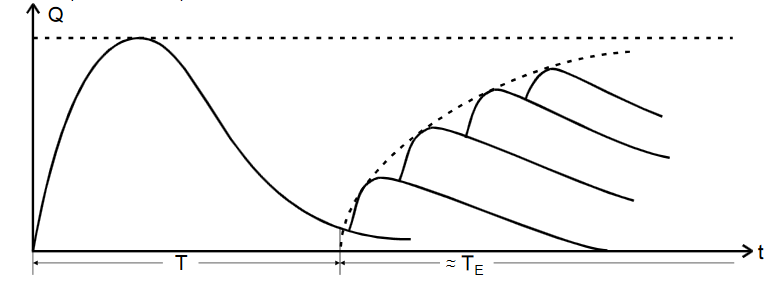
\includegraphics[width=\textwidth]{content/Totzeit.png}
  \caption{Tot- und Erholungszeit im Ladungs-Zeit-Diagramm.\cite{v703}}
  \label{fig:osz}
\end{figure}

Bei bekannter Ablenkgeschwindigkeit kann dann aus dem Bild die Totzeit abgeschätzt werden.
Bei der Zwei-Quellen-Methode wird zunächst ein Strahler mit dem Zählrohr vermessen. Anschließend wird ein zusätzlich ein zweiter Strahler
auf das Zählrohr gerichtet und die Messung wiederholt.
Zu guter letzt wird der erste Strahler entfernt und die Messung ein drittes mal durchgeführt.
Aus simpler Überlegung folgt für die gemessene Rate $N_\text{mess}$, die eigentliche Rate $N$ und die Totzeit $T$ allgemein:
\begin{equation}
    N = \frac{N_\text{mess}}{1-TN_\text{mess}}
\end{equation}
Und somit erhält man hier:
\begin{align}
    N_1     &= \frac{N_{1,\text{mess}}}{1-TN_{1,\text{mess}}} \\
    N_2     &= \frac{N_{2,\text{mess}}}{1-TN_{2,\text{mess}}}
\end{align}
\begin{align}
    N_{1+2} &= \frac{N_{1+2,\text{mess}}}{1-TN_{1+2,\text{mess}}} \\
            &= N_1 + N_2 \\
    \frac{N_{1+2,\text{mess}}}{1-TN_{1+2,\text{mess}}} &=\frac{N_{1,\text{mess}}}{1-TN_{1,\text{mess}}} + \frac{N_{2,\text{mess}}}{1-TN_{2,\text{mess}}}
\end{align}
Es ergibt sich für die Totzeit T näherungsweise:
\begin{equation}
    \label{eqn:totzeit}
    T \approx \frac{N_{1,\text{mess}} + N_{2,\text{mess}} - N_{1+2,\text{mess}}}{2N_{1,\text{mess}}N_{2,\text{mess}}}
\end{equation}

Die pro Event freigesetzte Ladung lässt sich über den mittleren Strom bestimmen.
Hierzu wird folgende Gleichung verwendet:
\begin{equation}
    \overline{I} = \frac{\symup{\Delta}Q}{\symup{\Delta}t} = \frac{\symup{\Delta}q N_\text{mess}}{\symup{\Delta}t}
\end{equation}
Somit folgt:
\begin{equation}
    \label{eqn:ladung}
    \symup{\Delta}q = \frac{\overline{I} \symup{\Delta} t}{N_\text{mess}}
\end{equation}
%\cite{sample}
